% !TEX root = ../main.tex
\section{Центральна гранична теорема}
\index{центральна гранична теорема}
Як було показано вище, для послідовності незалежних ВВ 
$\left\{ \xi_n\right\}_{n=1}^\infty$ зі скінченними математичними сподіваннями та обмеженими в сукупності
дисперсіями $\frac{1}{n}\sum\limits_{k=1}^n (\xi_k - \E\xi_k) \overset{\mathrm{P}}{\longrightarrow} 0$.
Виявляється, що якщо знаменник цих сум буде прямувати до $0$ повільніше, то границя (хоча й в слабшому сенсі) вже не буде нульовою.
\subsection{Теорема Ляпунова}
\begin{theorem*}[теорема Ляпунова]\label{CLT}\index{теорема!Ляпунова}
    Нехай $\left\{ \xi_n\right\}_{n=1}^\infty$ --- послідовність незалежних випадкових величин таких, 
    що існують скінченні $\E\xi_k = a_k$, $\D\xi_k = \sigma_k^2$ та
    $m_k = \E\left|\xi_k - a_k\right|^3$ і виконується умова Ляпунова: \index{умова!Ляпунова}
    \begin{gather*}
        \lim_{n \rightarrow \infty} \frac{\sum\limits_{k=1}^n m_k}{\left(
            \sum\limits_{k=1}^n \sigma_k^2
        \right)^{3/2}} = 0
    \end{gather*}
    Тоді рівномірно відносно $x$:
    \begin{gather}
        \lim_{n \rightarrow \infty} \P \left\{
            \frac{\sum\limits_{k=1}^n (\xi_k - a_k)}
            {\sqrt{\sum\limits_{k=1}^n \sigma_k^2}}
            < x
        \right\} = F_{\mathrm{N}(0, 1)}(x) = \Phi(x) + \frac{1}{2} = 
        \frac{1}{\sqrt{2\pi}} \int\limits_0^x e^{-\frac{t^2}{2}} dt + \frac{1}{2}
    \end{gather}
    або:
    \begin{gather*}
        \frac{\sum\limits_{k=1}^n (\xi_k - a_k)}
        {\sqrt{\sum\limits_{k=1}^n \sigma_k^2}}
        \overset{\mathrm{F}}{\longrightarrow} \xi \sim \mathrm{N}(0, 1),  \; n\to \infty
    \end{gather*}
\end{theorem*}
\begin{proof}
    Позначимо $\eta_n = \frac{\sum\limits_{k=1}^n (\xi_k - a_k)}
    {\sqrt{\sum\limits_{k=1}^n \sigma_k^2}}$, $\xi_k - a_k = \mathring{\xi_k}$ ($\E\mathring{\xi_k} = 0)$, 
    $B_n = \sqrt{\sum\limits_{k=1}^n \sigma_k^2}$. 
    Тоді $\eta_n = \frac{1}{B_n}\sum\limits_{k=1}^n \mathring{\xi_k}$.
    $\E\eta_n = 0$, $\D\eta_n = \frac{1}{B_n^2}\sum\limits_{k=1}^n \D\mathring{\xi_k} = 
    \left[\D\xi_k = \D\mathring{\xi_k}\right] = 1$.

    Доведення ґрунтується на теоремі Леві (\ref{levi_theor}): збіжність за розподілом послідовності 
    випадкових величин $\left\{ \xi_n\right\}_{n=1}^{\infty}$ еквівалентна поточковій збіжності їх
    характеристичних функцій.

    Нехай $\chi_k(t)$ --- характеристична функція $\mathring{\xi_k}$, а $F_k(x)$ --- 
    функція розподілу $\mathring{\xi_k}$.
    За властивостями характеристичних функцій $\chi_{\eta_n}(t) = 
    \prod\limits_{k=1}^n \chi_k(\frac{t}{B_n})$. 
    Доведемо, що $\chi_{\eta_n}(t)\to e^{-t^2/2} = 
    \chi_{\mathrm{N}(0, 1)}(t)$ при $ n \to \infty$.
    \begin{gather*}\chi_k\left(\frac{t}{B_n}\right) = \int\limits_{-\infty}^{+\infty} e^{i\frac{t}{B_n}x} dF_k(x) = 
    \int\limits_{-\infty}^{+\infty} \left(1 + i\frac{t}{B_n}x - \frac{t^2}{2B_n^2}x^2 - 
    i\frac{t^3}{6B_n^3}x^3 + ...\right) dF_k(x) = \\ = \left[\theta_k \in (0; 1)\right]
    = 1 + \frac{it}{B_n}\E\mathring{\xi_k} - \frac{t^2}{2B_n^2}
    \E\mathring{\xi_k}^2 + \theta_k\frac{|t|^3}{6B_n^3}\E|\mathring{\xi_k}|^3 = 
    1 - \frac{t^2}{2B_n^2}\sigma_k^2 + \theta_k\frac{|t|^3}{6B_n^3}m_k \\
    \ln\chi_{\eta_n}(t) = \sum\limits_{k=1}^n \ln \chi_k \left(\frac{t}{B_n}\right) = 
    \sum\limits_{k=1}^n \ln\left(1 - \frac{t^2}{2B_n^2}\sigma_k^2 + 
    \theta_k\frac{|t|^3}{6B_n^3}m_k\right)
    \end{gather*}

    З умови Ляпунова $\underset{n \rightarrow \infty}{\lim} \frac{\sum\limits_{k=1}^n m_k}{B_n^3} = 0$, 
    тому з відомої властивості $\ln(1 + \alpha_n) \sim \alpha_n$, де $\alpha_n$ --- нескінченно мала при 
    $n \rightarrow \infty$, маємо $\ln\chi_{\eta_n}(t) \sim \sum\limits_{k=1}^n\left(
        -\frac{t^2\sigma^2_k}{2B_n^2} + \theta_k\frac{|t|^3}{6B_n^3}m_k
    \right) 
    = -\frac{t^2}{2}\frac{\sum\limits_{k=1}^n\sigma_k^2}{B_n^2} + \sum\limits_{k=1}^n \theta_k\frac{|t|^3}{6B_n^3}m_k= -\frac{t^2}{2} 
    + \sum\limits_{k=1}^n \theta_k\frac{|t|^3}{6B_n^3}m_k \to -\frac{t^2}{2} 
    $ при $n \rightarrow \infty$.
    
    Таким чином, $\chi_{\eta_n}(t) \to e^{-\frac{t^2}{2}}$ при $n \rightarrow \infty$ і 
    з теореми Леві маємо, що $\eta_n \overset{\mathrm{F}}{\longrightarrow} \xi \sim \mathrm{N}(0, 1)$.
\end{proof}
\begin{remark}
    Можна довести, що для послідовності неперервних випадкових величин також має місце збіжність щільностей розподілу $\eta_n$ до $\frac{1}{\sqrt{2\pi}} e^{-\frac{x^2}{2}}$
    --- щільності розподілу $\mathrm{N}(0, 1)$.
\end{remark}
\noindent\textbf{Наслідок.} Нехай всі $\xi_n$ \emph{однаково розподілені}, $\E\xi_k = a$, $\D\xi_k = \sigma^2$,
$m_k = \E\left| \xi_k - a\right|^3 = m$. Тоді умова Ляпунова виконується автоматично:
$$\underset{n \rightarrow \infty}{\lim} \frac{\sum\limits_{k=1}^n m_k}{\left(
    \sum\limits_{k=1}^n \sigma_k^2
\right)^{3/2}} = \underset{n \rightarrow \infty}{\lim} \frac{n \cdot m}{(n\cdot \sigma^2)^{3/2}} = 0$$
В цьому випадку
$$\frac{\sum\limits_{k=1}^n (\xi_k - a_k)}
{\sqrt{\sum\limits_{k=1}^n \sigma_k^2}}
= \frac{1}{\sqrt{n}} \sum\limits_{k=1}^n \left( \frac{\xi_k - a}{\sigma}\right) \overset{\mathrm{F}}{\longrightarrow}\xi \sim \mathrm{N}(0, 1),
\;n \to \infty$$
Це твердження означає, що яким би не був розподіл $\xi_n$, $\xi_1 + ... + \xi_n$ матиме <<приблизно нормальний>> розподіл $\mathrm{N}(n a, n\sigma^2)$.
Проілюструємо це на прикладі рівномірного розподілу. На рисунку нижче зображено графіки щільностей розподілів
$\mathrm{U}[-1; 1]$ та $\mathrm{N}\left(0, \frac{1}{3}\right)$. Зауважимо, що $\frac{1}{3}$ --- це дисперсія $\mathrm{U}[-1; 1]$.
\begin{center}
    \begin{tikzpicture}[yscale = 5, xscale = 0.6]
        \pgfmathsetmacro{\a}{0};
        \pgfmathsetmacro{\s}{0.57735}
        \draw [->] (-5, 0) -- (5, 0);
        \draw [->] (0, -0.2) -- (0, 0.75);
        \draw [domain=-4.9:4.9, smooth, variable = \x, thick, gray] plot ({\x}, {0.398942280401/\s * e^(-(\x-\a)^2/(2*\s^2))});
        \node [below] at (5, 0) {$x$};
        \node [below right] at (0, 0) {$_0$};
        \node [below right] at (2, 0) {$_2$};
        \node [below left] at (-2, 0) {$_{-2}$};
        \node [below right] at (4, 0) {$_4$};
        \node [below left] at (-4, 0) {$_{-4}$};
        
        \draw [thick] (-1, 0.5) -- (1, 0.5);
        \draw [dashed] (-1, 0) -- (-1, 0.5);
        \draw [dashed] (1, 0) -- (1, 0.5);
        \draw [thick] (-5, 0) -- (-1, 0);
        \draw [thick] (1, 0) -- (4.9, 0);
    \end{tikzpicture}
\end{center}
Розглянемо тепер щільності розподілу сум двох (зліва) та трьох (справа) незалежних ВВ, кожна з яких має розподіл $\mathrm{U}[-1; 1]$, і щільності
нормальних розподілів $\mathrm{N}\left(0, \frac{2}{3}\right)$ та $\mathrm{N}\left(0, 1\right)$ відповідно.

\begin{center}
    \begin{tabular}{c c}
        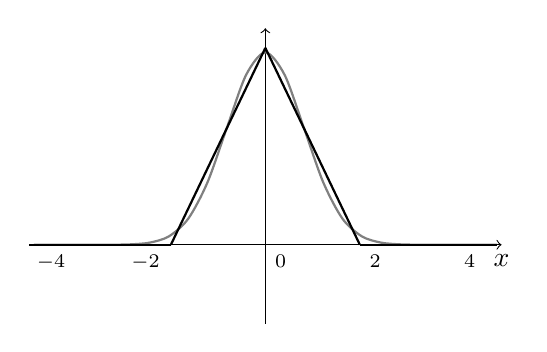
\begin{tikzpicture}[yscale = 5, xscale = 0.6]
            \pgfmathsetmacro{\a}{0};
            \pgfmathsetmacro{\s}{0.8165}
            \draw [->] (-5, 0) -- (5, 0);
            \draw [->] (0, -0.2) -- (0, 0.55);
            \draw [domain=-4.9:4.9, smooth, variable = \x, thick, gray] plot ({\x}, {0.398942280401/\s * e^(-(\x-\a)^2/(2*\s^2))});
            \node [below] at (5, 0) {$x$};
            \node [below right] at (0, 0) {$_0$};
            \node [below right] at (2, 0) {$_2$};
            \node [below left] at (-2, 0) {$_{-2}$};
            \node [below right] at (4, 0) {$_4$};
            \node [below left] at (-4, 0) {$_{-4}$};
            
            \draw [domain=-2:0, smooth, variable = \x, thick] plot ({\x}, {0.5 + \x/4});
            \draw [domain=0:2, smooth, variable = \x, thick] plot ({\x}, {0.5 - \x/4});
            \draw [thick] (-5, 0) -- (-2, 0);
            \draw [thick] (2, 0) -- (4.9, 0);
        \end{tikzpicture} &
        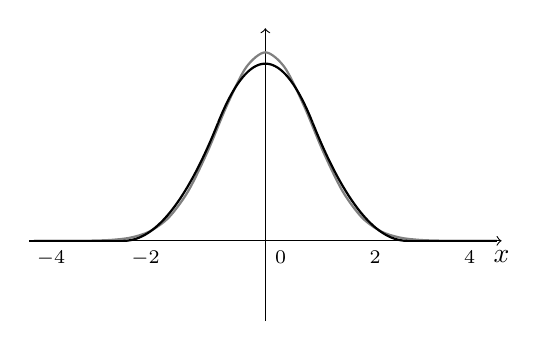
\begin{tikzpicture}[yscale = 6, xscale = 0.6]
            \pgfmathsetmacro{\a}{0};
            \pgfmathsetmacro{\s}{1}
            \draw [->] (-5, 0) -- (5, 0);
            \draw [->] (0, -0.17) -- (0, 0.45);
            \draw [domain=-4.9:4.9, smooth, variable = \x, thick, gray] plot ({\x}, {0.398942280401/\s * e^(-(\x-\a)^2/(2*\s^2))});
            \node [below] at (5, 0) {$x$};
            \node [below right] at (0, 0) {$_0$};
            \node [below right] at (2, 0) {$_2$};
            \node [below left] at (-2, 0) {$_{-2}$};
            \node [below right] at (4, 0) {$_4$};
            \node [below left] at (-4, 0) {$_{-4}$};
            
            \draw [domain=-3:-1, smooth, variable = \x, thick] plot ({\x}, {(3+\x)^2/16});
            \draw [domain=-1:0, smooth, variable = \x, thick] plot ({\x}, {3/8 - (\x)^2/8});
            \draw [domain=0:1, smooth, variable = \x, thick] plot ({\x}, {3/8 - \x^2/8});
            \draw [domain=1:3, smooth, variable = \x, thick] plot ({\x}, {(-3+\x)^2/16});
            \draw [thick] (-5, 0) -- (-3, 0);
            \draw [thick] (3, 0) -- (4.9, 0);
        \end{tikzpicture}
    \end{tabular}
\end{center}

Видно, що графік щільності суми трьох ВВ дуже схожий на графік щільності нормального розподілу $\mathrm{N}\left(0, 1\right)$.
\begin{exercise}
    Записати в явному вигляді щільності розподілу $\zeta_2 = \xi_1 + \xi_2$ та $\zeta_3 = \xi_1 + \xi_2 + \xi_3$, де
    $\xi_k \sim \mathrm{U}[-1; 1], k = 1,2,3$.
\end{exercise}
Варто пояснити практичне значення умови Ляпунова $\underset{n \rightarrow \infty}{\lim} \frac{\sum\limits_{k=1}^n \E\left| \xi_k - \E\xi_k\right|^3}{\left(
    \sum\limits_{k=1}^n \D\xi_k
\right)^{3/2}} = 0$ в доведенні теореми. Вона означає, що дисперсії величин у послідовності мають бути приблизно однакового порядку. 
Можна навести приклад з життя: якщо в багатоквартирному будинку не буде квартири, що використовує значно більше електроенергії, ніж інші,
то сумарний розподіл кількості використаної електроенергії буде приблизно нормальним.

\subsection{Умова Ліндеберга}\index{умова!Ліндеберга}
    Замість умови Ляпунова в доведенні однойменної теореми \ref{CLT} можна вимагати виконання умови Ліндеберга:
    $$\forall \; \varepsilon > 0 : \underset{n\to\infty}{\lim} 
    \frac{1}{B_n^2}\sum\limits_{k=1}^n \E \left( \left( \xi_k - a_k\right)^2 \cdot \mathds{1}{\left\{|\xi_k - a_k| > \varepsilon \cdot B_n\right\}}\right) = 0$$
    Тут $a_k = \E\xi_k$, $B_n = \sqrt{\sum\limits_{k=1}^n \D\xi_k}$, $\mathds{1} A$ --- індикатор події $A$.
    Ймовірнісний зміст цієї умови такий: нехай $A_k = \left\{ \left|\xi_k - a_k \right| > \varepsilon \cdot B_n \right\}$, тоді
    \begin{gather*}
        \P \left( \bigcup\limits_{k=1}^n A_k\right) \leq \sum\limits_{k=1}^n \P(A_k) = \sum\limits_{k=1}^n \int_{|x-a_k| > \varepsilon \cdot B_n} dF_k(x) \leq
    \sum\limits_{k=1}^n \int_{|x-a_k| > \varepsilon \cdot B_n} \frac{(x-a_k)^2}{\varepsilon^2 B_n^2} dF_k(x) = \\
    = \frac{1}{\varepsilon^2} \cdot \frac{1}{B_n^2}\sum\limits_{k=1}^n \E \left( \left( \xi_k - a_k\right)^2 \cdot \mathds{1}{\left\{|\xi_k - a_k| > \varepsilon \cdot B_n\right\}}\right) 
    \to 0, \; n\to\infty
    \end{gather*}
    Це означає, що кожний доданок $\frac{\xi_k - a_k}{B_n}$ має рівномірно малий внесок в суму $\frac{1}{B_n}\sum\limits_{k=1}^n (\xi_k - a_k)$.
Повне доведення ЦГТ з умовою Ліндеберга виходить за рамки курсу.